\chapter{Évolution Différentielle sur les circuits simple et double diodes}

\section{Introduction}
Maintenant que nous avons abordé les modèles à diodes et l'Évolution Différentielle indépendemment l'un de l'autre, dans ce chapitre nous allons appliquer l'ED \nomenclature{ED}{Évolution Differentielle (\textit{Differential Evolution})} sur les modèles pour estimer les valeurs des paramètres en utilisant les données expérimentales standards de la littérature. En ce qui concerne l'implémentation pratique de cette technique, on utilise le langage de programmation \textit{Python}. On fait appel a quelques bibliothèques scientifiques de Python pour fournir les outils mathématiques requis par la méthode. A partir d'ici nous allons fournir des petits extraits de code pertinents à la discussion qui montrent la manière d'implémenter les étapes de la méthode. Pour des raisons de clarté ce ne sont pas des extraits complètement fidèles au code utilisé en réalité. Le code complet et non modifié est disponible comme annexe à la fin de ce document. 

\section{Fonction W de Lambert}
Les méthodes évolutionnaires dépendent d'une fonction objectif qu'il faut minimiser, pour sélectionner les meilleures solutions dans une population. Dans notre cas, la fonction objectif est la \textit{RMSE} \nomenclature{RMSE}{Racine de l'erreur quadratique moyenne (\textit{Root Mean Squared Error})} et elle quantifie la différence entre la courbe caractéristique du modèle et les données expérimentales. Cependant, chaque fois qu'un vecteur solution $\vec{V}$ (formules \ref{eq:vsol}) est généré, il faut pouvoir recréer la courbe I-V associée pour permettre à la fonction objectif de calculer la RMSE.
\begin{equation}
  \label{eq:vsol}
  \vec{V}_{\text{simple diode}} = 
  \begin{bmatrix}
    R_s\\
    R_{p}\\
    a\\
    I_0\\
    I_{PV}
  \end{bmatrix},
  \quad
  \vec{V}_{\text{double diode}} = 
  \begin{bmatrix}
    R_s\\
    R_{p}\\
    a_1\\
    a_2\\
    I_{01}\\
    I_{02}\\
    I_{PV}
  \end{bmatrix}
\end{equation}
On pourrait implémenter la fonction objectif en code de la manière suivante:\\

\noindent
\begin{minipage}{\linewidth}
\begin{minted}[mathescape,
               linenos,
               numbersep=5pt,
               gobble=2,
               frame=lines,
               framesep=2mm,
               breaklines=true,
               fontsize=\scriptsize]{Python}
    # Cette fonction prend un vecteur solution et les points IV expérimentaux comme arguments
    def objf(vecteur, exp_v, exp_i):
        # Pénalisons le vecteur si les valeurs sont non-physiques
        rs, rp = vecteur[0], vecteur[1]
        if rs < 0 or rp < 0:
            return 100 # Valeur fitness large
        ical = i_from_vect(vector, exp_v) # Une fonction donnant la caractéristique IV de "vector"
        erreur = ical - exp_i
        return np.sqrt(np.mean(erreur ** 2)) # RMSE         
\end{minted}
\end{minipage}
\vspace*{12pt}

Les équations de modèles simple et double diode (équations \ref{eq:single}, \ref{eq:doublediode}, respectivement) sont transcendantes, il est donc impossible d'extraire directement le courant à partir de la tension et des paramètres (Le courant $I$ figure simultanément dans le premier membre et dans l'exponentiel du second). Ainsi, il n'est pas trivial de remplir la fonction de \pyth{i_from_vect(vector, exp_vol)}. Plusieurs méthodes on été utilisées initialement avec des approches d'approximation analytique ou itérative \cite{Shur1991,AbuelmaAtti1992,Datta1992}. Ces méthodes sont approximatives mais permettent de trouver la solution explicitement avec des fonctions élémentaires (Développement Taylor par exemple). Dans notre cas, on fait recours à la méthode de Jain et Kapoor (2004) \cite{Jain2004, Lun2015} qui utilisent la fonction W de Lambert pour une solution analytique exacte de ces équations.

\subsection{Définition}
La "\textit{fonction W}" de Lambert est définie comme l'inverse de la fonction $w \rightarrow f(w) =  w e^w$, où $w = W_k(z)\ |\ z \in \mathbb{C}$. La fonction $f$ n'étant pas surjective, la fonction $W_k(z)$ est donc \textit{multivaluée} et comprends plusieurs branches indexées par $k$ ($W_0$ est choisie comme branche principale). Si $x \in \mathbb{R}$ et $-1/e \leq x < 0$, il existe deux valeurs réelles possible de $W(x)$ (figure \ref{fig:lambertw}).

\begin{figure} 
  \begin{center}
    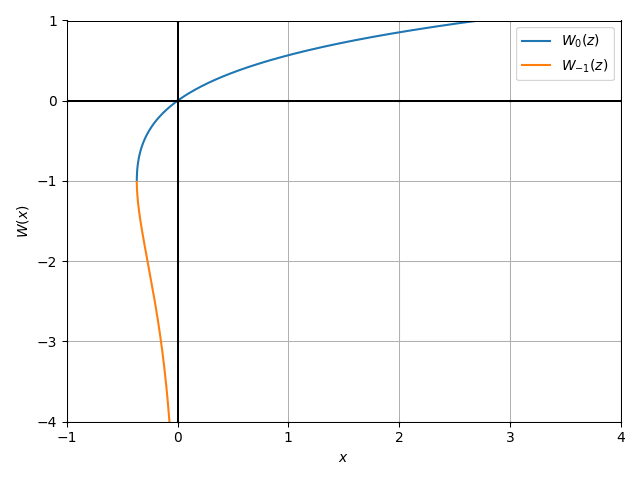
\includegraphics[width=.6\textwidth]{resources/lambertw.png}
    \caption{Les deux branches réelles de $W(x)$ lorsque $x$ est réel}
    \label{fig:lambertw}
  \end{center}
\end{figure}

\subsection{Évaluation de la fonction $W$}

Le fait qu'il n'existe pas de fonctions mathématiques élémentaires donnant explicitement $W(z)$ est remédié par l'existence de plusieurs \textit{algorithmes de recherche des zéros} permettant le calcul des valeurs de n'importe quelle branche de la fonction $W$. Dans notre cas spécifique, la bibliothèque scientifique \textit{scipy} de Python fournit une fonction W implémentée par l'itération de Halley qui est un exemple d'une méthode de classe "Householder"\footnote{La méthode de Newton est un exemple d'une méthode de Householder}. La méthode de Halley a été appliquée à la fonction $W$  par Corless et al. \cite{Corless1996} donnant:
\begin{equation}
  \label{eq:halley}
  w_{j+1} = w_j - \frac{w_j e^{w_j} - z}{e^{w_j}(w_j + 1) - \frac{(w_j + 2)(w_j e^{w_j} - z)}{2w_j + 2}}
\end{equation}

Un exemple basique de l'utilisation de cette méthode en Python est le suivant:\\

\noindent
\begin{minipage}{\linewidth}
\begin{minted}[mathescape,
               linenos,
               numbersep=5pt,
               gobble=2,
               frame=lines,
               framesep=2mm,
               fontsize=\footnotesize]{Python}
  import numpy as np 
  from scipy.special import lambertw # scipy fournit la fonction W

  z = np.linspace(-1/np.e, 3, 1000) # evaluons W entre -1/e et 3
  w0 = lambertw(z, 0) # choisir la branche principale
\end{minted}
\end{minipage}

\subsection{Résolution des modèles simple et double diode par la fonction W}
Depuis la définition de la fonction W, la solution d'une équation $xe^x = a$ est $x = W(a)$. En effectuent des manipulations algébriques élémentaires sur le modèle simple diode (equation \ref{eq:single}), Jain et Kapoor ont montré que l'expression explicite du courant en fonction des paramètres et de la tension est:
\begin{equation}
  \label{eq:lambertwsingle}
  I = \frac{R_{sh}(I_0 + I_{PV}) - V}{R_s + R_{sh}} - \frac{W\left(\frac{R_s I_0 R_{sh}}{a V_{th}(R_s + R_{sh})}e^{\left(\frac{R_{sh}(R_s I_{PV} + R_s I_0 + V)}{a V_{th} (R_s + R_{sh})}\right)}\right)aV_{th}}{R_s}
\end{equation}
On remarque bien que le second membre ne contient nul part un terme de courant $I$. Il faut noter aussi que le terme de la fonction $W$ est sous risque d'un dépassement et de retourner des valeurs infinies. Pour des raisons de stabilité numérique on utilise la notion de \textit{Conductance Shunt}: $C_{sh} = \frac{1}{R_{sh}}$ car cette résistance prend souvent de valeurs $\gg 1$ ce qui entraîne un risque de divergence des calculs. On trouve souvent des valeurs larges de résistance shunt, ce qui explique l'existence dans la littérature de plusieurs modèles utilisant la simplification $R_{sh} = + \infty$. Avec la substitution de la conductance shunt, si $R_{sh}\rightarrow\infty$ alors $C_{sh} \rightarrow 0$ ce qui assure la stabilité du calcul numérique.

Le modèle double diodes (équation \ref{eq:doublediode}) contient un terme exponentiel pour chaque diode. De la même manière que Jain et Kapoor on retrouve explicitement l'expression du courant avec deux termes de la fonction $W$ (equation \ref{eq:lambertwdouble}).
\begin{equation}
  \label{eq:lambertwdouble}
  \begin{split}
    I &= \frac{R_{sh} (I_{01} + I_{02} + I_{PV}) - V}{R_s + R_{sh}}\\ 
    &- \frac{a_1}{2 R_s} W\left( \frac{R_s R_{sh}(I_{01} + I_{02})}{a_1 (R_s + R_{sh})}e^{\left(\frac{R_{sh}(R_s I_{PV} + R_s I_{01} + R_s I_{02} + V)}{a_1 (R_s + R_{sh})}\right)}\right)\\ 
    &- \frac{a_2}{2 R_s} W\left( \frac{R_s R_{sh}(I_{01} + I_{02})}{a_1 (R_s + R_{sh})}e^{\left(\frac{R_{sh}(R_s I_{PV} + R_s I_{01} + R_s I_{02} + V)}{a_2 (R_s + R_{sh})}\right)}\right)
  \end{split}
\end{equation}

\section{Utilisation de l'outil \textit{DEPV}}

\nomenclature{$F$}{Facteur de mutation}
\nomenclature{$CR$}{Taux de croisement}
\nomenclature{$N_P$}{Taille de la population}
%\nomenclature{$Gen_{max}$}{Nombre maximal de générations}
\nomenclature{$D$}{Dimensions de l'espace de recherche}
Pour appliquer l'Évolution Différentielle avec succès sur les modèles à diodes, il faut savoir choisir les bonnes valeurs de paramètres de contrôle $CR, F \text{et}\  N_P$. Il n'existe pas de règle stricte mais Storn et Price \cite{Price2005} donnent quelques indications. En ce qui concerne le facteur de mutation $F$, les valeurs $F \geq 1$ ne sont pas fiables et souvent convergent très lentement par rapport aux $F < 1$. Cependant, Zaharie (2002) \cite{Zaharie2002} constate une borne inférieure de $F > 0.4$. Puisque l'opération de \textit{sélection} tend à réduire la diversité dans la population, le rôle de la \textit{mutation} et de balancer cette pression exercée sur la population et tend à augmenter la diversité. Si $F$ est trop petit, l'ED peut converger même avec l'absence de la pression sélective. En ce qui concerne le taux de croisement $CR$, Salomon (1996) \cite{Salomon1996} a démontré les limites d'un $CR$ trop petit et par conséquent Storn et Price recommandent des valeurs de $CR$ proche de $1$. Reste à choisir la taille de la population $N_P$, généralement $10D \leq N_P \leq 20D$ est recommandé mais dans notre cas on optera à $N_P = 100$.

Dans ce projet, nous avons développé une bibliothèque en Python fournissant une interface permettant de lancer des calculs avec la technique de l'ED sur n'importe quelles cellule, à condition d'avoir accès aux données expérimentales. On fournit la fonction \pyth{read_csv()} qui permet à l'utilisateur d'extraire les points expérimentaux de la caractéristique IV (voltage en abscisses et courant en ordonnées) à partir d'un fichier .txt ou .csv. Nous fournissons aussi une classe \pyth{DE} qui gère tous les calculs. Il suffit de lui donner les paramètres nécessaires tel que les bornes de l'espace de recherche et le fichier contenant les données expérimentales. Pour plus de contrôle sur les paramètres de l'algorithme, la classe \pyth{DE} expose plusieurs variable à travers son "constructeur". Le prototype de la fonction constructrice ou \pyth{__init__()} est le suivant:

\begin{minted}[mathescape,
               linenos,
               numbersep=5pt,
               gobble=2,
               frame=lines,
               framesep=2mm,
               breaklines=true,
               fontsize=\scriptsize]{Python}
    def __init__(self, bounds, ivdata, Ns, Np, temp, popsize=100, maxiter=200, mutf=0.7, crossr=0.8):
        """
        :param bounds: Dictionary of bounds in this form {'rp': [lower, upper], 'rs': [lower, upper] ...}
        :param ivdata: [Voltages, Currents]
        :param Ns: Number of cells in series
        :param Np: Number of cells in parallel
        :param temp: Temperature
        :param popsize: Population size
        :param maxiter: Maximum number of generations
        :param mutf: Mutation Factor F
        :param crossr: Crossover Rate CR
        """
\end{minted}
Notons les valeurs prise par défaut pour la taille de la population $N_P = 100$, le nombre de générations maximal $Gen_{max} = 200$, le facteur de mutation $F = 0.7$ et le taux de croisement $CR = 0.8$. Si l'utilisateur ne fournit pas explicitement ces paramètres, les valeurs par défaut sont alors utilisées.
Un exemple d'exécution de la classe DE sur la cellule est le suivant:
\begin{minted}[mathescape,
               linenos,
               numbersep=5pt,
               gobble=2,
               frame=lines,
               framesep=2mm,
               fontsize=\scriptsize]{Python}
  # On importe la classe DE et la fonction read_csv()
  from objects import DE, read_csv

  # Bornes de l'espace de recherche
  bornes = {'rp':  [2, 100],
            'rs':  [0, 1],
            'a':   [1, 2],
            'i0':  [1e-07, 1e-04],
            'ipv': [0, 10]}
  
  # Température en K et nombre de cellules en serie et en parallele
  T = 33 + 275.15
  Ns, Np = 1, 1

  # Données expérimentales disponible dans un fichier .csv
  exp = read_csv("data/RTC33D1000W.csv")

  # On crée un objet DE pour utiliser ces données et effectuer le calcul
  RTC = DE(b, exp, Ns, Np, T)

  # On lance le calcul
  RTC.solve()

  # Traçage des graphes et résultats
  RTC.plot_fit_hist()
  RTC.plot_result(print_params=True)
\end{minted}
Si on veut utiliser le modèle double diode, il suffit de donner 7 intervalles au lieu de 5 comme premier argument. DEPV reconnaît automatiquement le modèle à utiliser à partir de la taille du dictionnaire \pyth{bornes} fournit à la classe \pyth{DE}:
\begin{minted}[mathescape,
               linenos,
               numbersep=5pt,
               gobble=2,
               frame=lines,
               framesep=2mm,
               fontsize=\scriptsize]{Python}
  bornes = {'rp':  [2, 100],
       'rs':  [0, 1],
       'a1':  [1, 2],
       'a2':  [1, 2],
       'i01': [1e-7, 1e-5],
       'i02': [1e-7, 1e-5],
       'ipv': [0, 5]}
       
  T = 45 + 275.15
  Ns, Np = 36, 1
  exp = read_csv("data/PWP.csv")
  PWP = DE(bornes, exp, Ns, Np, T)
  PWP.solve()
  PWP.plot_result(print_params=True)
\end{minted}
Dans le cas où on n'a pas besoin d'accéder à cette fonctionnalité programmatiquement, il suffit d'utiliser directement l'interface graphique de DEPV. On a toujours besoin de fournir le fichier contenant les données expérimentales, la température, les bornes et les cellules en série et en parallèle (figure \ref{fig:depvmain}). Les résultats et les graphes sont affichés par l'interface dans la figure \ref{fig:depvres}

\begin{figure}[H]
  \begin{center}
    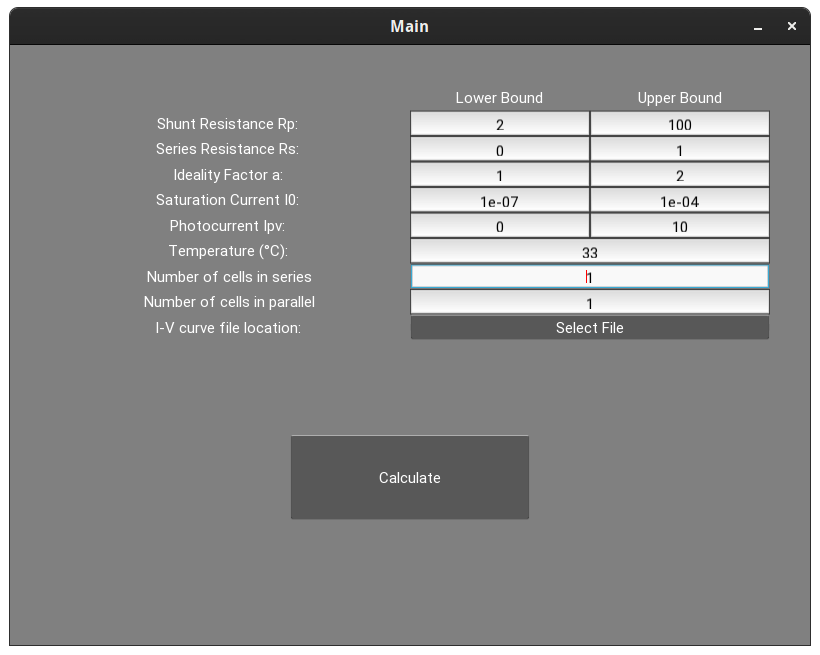
\includegraphics[width=0.7\textwidth]{resources/paramwindow.png}
    \caption{Interface principale de l'outil DEPV avec les champs texte pour insérer les bornes, la température, les cellules en séries/parallèle et le fichier .csv contenant les données expérimentales}
    \label{fig:depvmain}
  \end{center}
\end{figure}

\begin{figure}[H]
  \begin{center}
    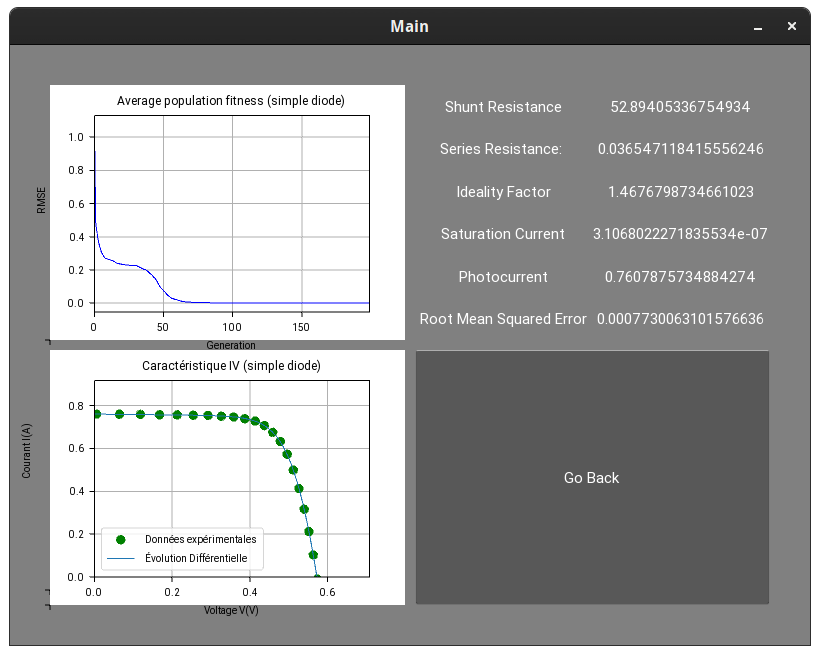
\includegraphics[width=0.7\textwidth]{resources/reswindow.png}
    \caption{Graphes et résultats affichés par DEPV pour la cellule RTC France 57 mm}
    \label{fig:depvres}
  \end{center}
\end{figure}

\section{Stratégie métaheuristique}
Comme on l'a déjà mentionné, la sélection des paramètres de l'ED, notamment le Facteur de Mutation $F$ et le taux de croisement $CR$, reste assez arbitraire et empirique malgré son influence déterminante sur la convergence de la technique. Bien que Storn et Price \cite{Price2005} recommandent des valeurs de $F$ proche de $1$ et que les limites déterminées par Zaharie et al. \cite{Zaharie2002} sont souvent correctes, il existe des cas atypiques comme l'estimation des états fondamentaux des agrégats $Si_{x}-H$ par Chakraborti et al. (2001) \cite{Chakraborti2001}. Dans leur cas, l'ED a réussi à minimiser l'énergie des agrégats atomiques avec des facteurs de mutation entre $0.0001$ et $0.4$.

On propose donc une technique métaheuristique permettant de déterminer ces paramètres sans faire recours à l'arbitraire/l'empirique. Cette solution consiste à utiliser l'ED à un niveau plus haut pour déterminer les paramètres à utiliser pour l'ED usuelle pour l'estimation des paramètres comme on a décrit dans le chapitre précèdent. Le nouvel espace de recherche est donc à deux dimensions seulement ($F$ et $CR$) et par conséquent n'a besoin que d'une population de $10 \times D = 20$ vecteurs solutions. En effet, chaque vecteur solution représente une instance entière d'Évolution Différentielle avec des $F$ et $CR$ différents. La fonction objectif est simplement la valeur fitness du meilleur résultat obtenu avec un $F$ et $CR$ spécifique. Il est vrai que cette technique apparaît très coûteuse en termes de calcul, puisque dans ce cas, chaque vecteur solution ne pourra être évalué qu'après sa propre instance d'ED ait convergé. Dans l'ED "standard" décrite dans le chapitre 2, une instance effectue $N_P \times Gen_{max} = 100 \times 200 = 20000$ évaluations de la fonction objectif. Avec cette ED "d'ordre supérieur", le nombre d'évaluations sera $N_{P}^{\text{higher order}} \times Gen_{max}^{\text{higher order}} \times 20000$. Ce qui correspond à $\num{2e6}$ évaluations pour $N_{P}^{\text{higher order}} = 20$ et  $Gen_{max}^{\text{higher order}} = 50$. En revanche, une seule exécution de cette technique au préalable et nécessaire. Les valeurs obtenues avec cette technique peuvent par la suite être réutilisées plusieurs fois avec l'ED standard et seulement les 20000 évaluations. Le nature coûteuse de cette technique est donc moins problématique puisque elle n'est utile que dans les cas où les ressources en capacité de calcul et en temps ne sont pas déterminantes. Par ailleurs, l'utilisation de cette technique permet de choisir les paramètres optimaux et donc à accélérer la convergence pour les cas où la rapidité des calculs est effectivement essentielle (Estimation des paramètres en temps réel par exemple). Le pseudo-code de cette technique est présenté dans l'algorithme \ref{alg:metaheuristic}. Notons que dans la ligne 26, l'évaluation de la fonction objectif $f(V_{j,gen})$ contient une instance entière de l'algorithme \ref{alg:debestbin} avec le facteur de mutation et taux de croisement fournis par le vecteur $V_{j,gen}$.

\begin{algorithm}[H]
  $CR^{\text{higher order}} \gets$ Taux de croisement\;
  $D^{\text{higher order}} \gets$ Dimensions de l'espace de recherche (2 dans ce cas)\;
  $N_{P}^{\text{higher order}} \gets$ Nombre de population ($10 \times D$)\;
  $gen = 0$\;
  Initialisation de la population $P_0 = [V_0, V_1, .., V_{N_P}]$\;
  \For{$i = 0 \text{\ to\ } N_P$}{
    $V_{min} = [V_{F,min}, V_{CR,min}]$\;
    $V_{max} = [V_{F,max}, V_{CR,max}]$\;
    $V_{i} = V_{min} + \text{rand}[0, 1] (V_{max} - V_{min})$\;
  }
  \While{$gen < gen_{max}$}{
    \For{$j = 0$\ to\ $N_P$}{
      $V_{j,gen} = [V_{F,j,gen}, V_{CR,j,gen}]$\;
      Choisir le vecteur de base et deux vecteurs aléatoires $V_{r1}\ \text{et}\ V_{r2} \in P_{gen}$\;
      $V_{base} = V \in P_{gen} \mid \forall (K \in P_{gen}), \quad f(V) \leq f(K)$\;
      Mutation :\\
      $M_{j,gen} = V_{base} + F^{\text{higher order}} (V_{r1} - V_{r2})  $\;
      Croisement : \\
      $T_{j,gen} = [T_{F,j,gen}, T_{CR,j,gen}]$\;
      \eIf{rand$[0, 1] < CR^{\text{higher order}}\ $ or\ $j = j_{rand}$}{
        $T_{i,j,gen} = M_{i,j,gen}$\;
      }{
        $T_{i,j,gen} = V_{i,j,gen}$\;
      }
      Sélection :\\
      \eIf{$f(T_{j,gen}) < f(V_{j,gen})$}{
        $V_{j,gen + 1} = T_{j, gen}$\;
      }{
      $V_{j,gen + 1} = V_{j, gen}$\;
      }
    }
      $gen = gen + 1$\;
  }
  \caption{Stratégie métaheuristique pour déterminer $F$ et $CR$}
  \label{alg:metaheuristic}
\end{algorithm}

\section{Conclusion}
